% !TeX program = pdflatex
\documentclass[11pt,a4paper]{article}
\usepackage[T1]{fontenc}
\usepackage[utf8]{inputenc}
\usepackage{lmodern}
\usepackage{microtype}
\usepackage[main=turkish, english]{babel}
\usepackage{geometry}
\geometry{margin=2.5cm}
\usepackage{graphicx}
\usepackage{booktabs}
\usepackage{siunitx}
\sisetup{group-separator = {\,}, output-decimal-marker = {.}}
\usepackage[unicode]{hyperref}
\PassOptionsToPackage{hyphens}{url}
\hypersetup{
  colorlinks=true,
  linkcolor=black,
  citecolor=black,
  urlcolor=blue,
  pdftitle={IzmirWildfire2025: Sentinel-2 ile NDVI/NBR Tabanlı Yangın Etki Analizi},
  pdfauthor={Yusuf Talha ARABACI}
}
\usepackage{caption}
\usepackage{subcaption}
\usepackage{amsmath}
\usepackage{float}
\usepackage[section]{placeins}

\title{IzmirWildfire2025: Sentinel-2 ile NDVI/NBR Tabanlı Yangın Etki Analizi}
\author{Yusuf Talha ARABACI\\Karabük Üniversitesi\\Yüksek Lisans, Yazılım Mühendisliği Öğrencisi}
\date{\today}

\begin{document}
\selectlanguage{turkish}
\sloppy
\maketitle
\thispagestyle{empty}

\begin{abstract}
Bu çalışma, 2025 İzmir orman yangınının etkilerini Sentinel-2 L2A verileri ile NDVI ve NBR endekslerine dayalı olarak incelemektedir. Önce-sonra dönemlerine ait median kompozitler üzerinde NDVI/NBR ve fark endeksleri (dNDVI, dNBR) hesaplanmış; dNBR eşiklerine göre şiddet sınıflandırması üretilmiştir. Deniz ve kıyı kaynaklı yalancı değişimleri azaltmak üzere SCL tabanlı su maskesi, NDWI/MNDWI denetimi, kıyı tamponu ve yanıcı yüzey filtresi (pre NDVI > 0.25) uygulanmıştır. Bulgular doğal renk (RGB) ve tematik haritalar ile özet tablolar eşliğinde sunulmuştur.
\end{abstract}

\noindent\textbf{Anahtar Kelimeler:} Sentinel-2, NDVI, NBR, dNBR, yanıklık şiddeti, uzaktan algılama, İzmir.

\tableofcontents
\clearpage

\section{Giriş}
Yangınların ekosistem, toprak ve yerleşimler üzerindeki etkilerinin nicel ve mekânsal olarak ortaya konması; yangın sonrası rehabilitasyon, yeniden ormanlaştırma ve risk azaltma planlamaları açısından kritik öneme sahiptir. Uzaktan algılama, yüksek zamansal ve mekânsal çözünürlükte tekrarlanan gözlemler üzerinden önce-sonra karşılaştırmalarına imkân tanır. Bu çalışmada Sentinel-2 L2A verileriyle NDVI ve NBR endekslerine dayalı bir yaklaşım sunulmakta; dNDVI ve dNBR ile etki/şiddet haritaları üretilmektedir.

\section{Çalışma Alanı (AOI)}
Çalışma alanı İzmir ili sınırları içinde belirlenmiştir. AOI, deponun \texttt{gee/aoi.geojson} dosyasında çokgen (Polygon) olarak tanımlıdır ve analizler bu AOI üzerinde yürütülmüştür.

\section{Veri ve Yöntem}
\subsection{Veri Kaynakları ve Dönemler}
\begin{itemize}
  \item \textbf{Uydu verisi:} Sentinel-2 L2A (10--20 m). NDVI için B8 (NIR), B4 (Kırmızı); NBR için B8 (NIR), B12 (SWIR2).
  \item \textbf{Platform:} Google Earth Engine (GEE) Python API.
  \item \textbf{Dönemler:} Öncesi: 2025-06-01 -- 2025-06-10; Sonrası: 2025-08-20 -- 2025-08-30.
\end{itemize}

\subsection{Ön İşleme ve Maskeleme}
Önce-sonra aralıkları \texttt{COPERNICUS/S2\_SR\_HARMONIZED} koleksiyonundan AOI ve tarih filtresiyle seçilmiştir. QA60 (bulut/sirrus) maskesi, SCL su sınıfı (6) ve NDWI/MNDWI kontrolleriyle su/deniz alanları dışlanmıştır. Kıyı şeridi etkilerini azaltmak için su maskesi çevresinde \SI{100}{m} kıyı tamponu uygulanmış; yanıcı olmayan yüzeyleri dışlamak için \emph{burnable} koşulu (pre NDVI $>0.25$) kullanılmıştır. Her dönem için median kompozit üretilmiştir.

\subsection{Endeksler ve Farklar}
NDVI $=(\mathrm{NIR}-\mathrm{Red})/(\mathrm{NIR}+\mathrm{Red})$, NBR $=(\mathrm{NIR}-\mathrm{SWIR2})/(\mathrm{NIR}+\mathrm{SWIR2})$ olarak tanımlanmıştır. Fark endeksleri \(\mathrm{dNDVI}=\mathrm{post}-\mathrm{pre}\), \(\mathrm{dNBR}=\mathrm{pre}-\mathrm{post}\) biçiminde hesaplanmıştır. Bu tanıma göre vejetasyon kaybı dNDVI$<0$, yanıklık artışı dNBR$>0$ ile ifade edilir.

\subsection{Şiddet Sınıflandırması ve Eşikler}
dNBR için 0--4 arası sınıflar USGS-benzeri eşiklerle (\(t_0=0.10, t_1=0.27, t_2=0.44, t_3=0.66\)) üretilmiştir. Çalışmada \texttt{gee/change.py} içinde sınıflandırma parametreleştirilmiş olup AOI'ye göre eşikler uyarlanabilmektedir.

\subsection{Uygulama ve Depo Yapısı}
Kodlar \texttt{gee/} altında düzenlenmiştir: \texttt{pipeline.py} (uçtan uca akış), \texttt{preprocess.py} (maskeleme/kompozit), \texttt{indices.py} (NDVI/NBR/NDWI/MNDWI), \texttt{change.py} (dNDVI/dNBR, sınıflandırma), \texttt{visualize.py} (harita/PNG/istatistik). Çıktılar \texttt{results/} klasöründe HTML/PNG/CSV olarak üretilmiştir. Web sunumu için depo kökündeki \texttt{index.html} kullanılmaktadır.

\section{Sonuçlar}
\subsection{Özet İstatistikler}
Aşağıdaki tablo, bu çalışmada hesaplanan özet ölçütleri (3 ondalık) göstermektedir.
\begin{table}[H]
  \centering
  \begin{tabular}{@{}ll@{}}
  \toprule
  Ölçüt & Değer \\
  \midrule
  NDVI (Önce) ort. & \num{0.451} \\
  NDVI (Sonra) ort. & \num{0.431} \\
  dNDVI ort. & \num{-0.022} \\
  dNBR ort. & \num{0.003} \\
  \bottomrule
  \end{tabular}
  \caption{Özet istatistikler (statik değerler).}
\end{table}

\subsection{Şiddet Alanları}
Şiddet sınıflarına göre alan dökümü (hektar) Tablo~\ref{tab:areas}'da verilmiştir.
\begin{table}[H]
  \centering
  \begin{tabular}{@{}ll@{}}
  \toprule
  Sınıf & Alan [ha] \\
  \midrule
  Yanıksız/Düşük (0) & \num{290265.14} \\
  Düşük (1) & \num{26482.59} \\
  Orta--Düşük (2) & \num{7166.76} \\
  Orta--Yüksek (3) & \num{6015.47} \\
  Yüksek (4) & \num{5783.67} \\
  Toplam yanmış alan & \num{45448.49} \\
  \bottomrule
  \end{tabular}
  \caption{dNBR şiddet sınıflarına göre alanlar.}
  \label{tab:areas}
\end{table}

\subsection{Haritalar}
\begin{figure}[H]
  \centering
  \begin{subfigure}[b]{0.48\textwidth}
    \centering
    \includegraphics[width=\linewidth]{../results/pre_RGB.png}
    \caption{Öncesi RGB (B4,B3,B2)}
  \end{subfigure}\hfill
  \begin{subfigure}[b]{0.48\textwidth}
    \centering
    \includegraphics[width=\linewidth]{../results/post_RGB.png}
    \caption{Sonrası RGB (B4,B3,B2)}
  \end{subfigure}
  \caption{Doğal renk (RGB) karşılaştırması.}
  \label{fig:rgb}
\end{figure}
\FloatBarrier

\begin{figure}[H]
  \centering
  \begin{subfigure}[b]{0.48\textwidth}
    \centering
    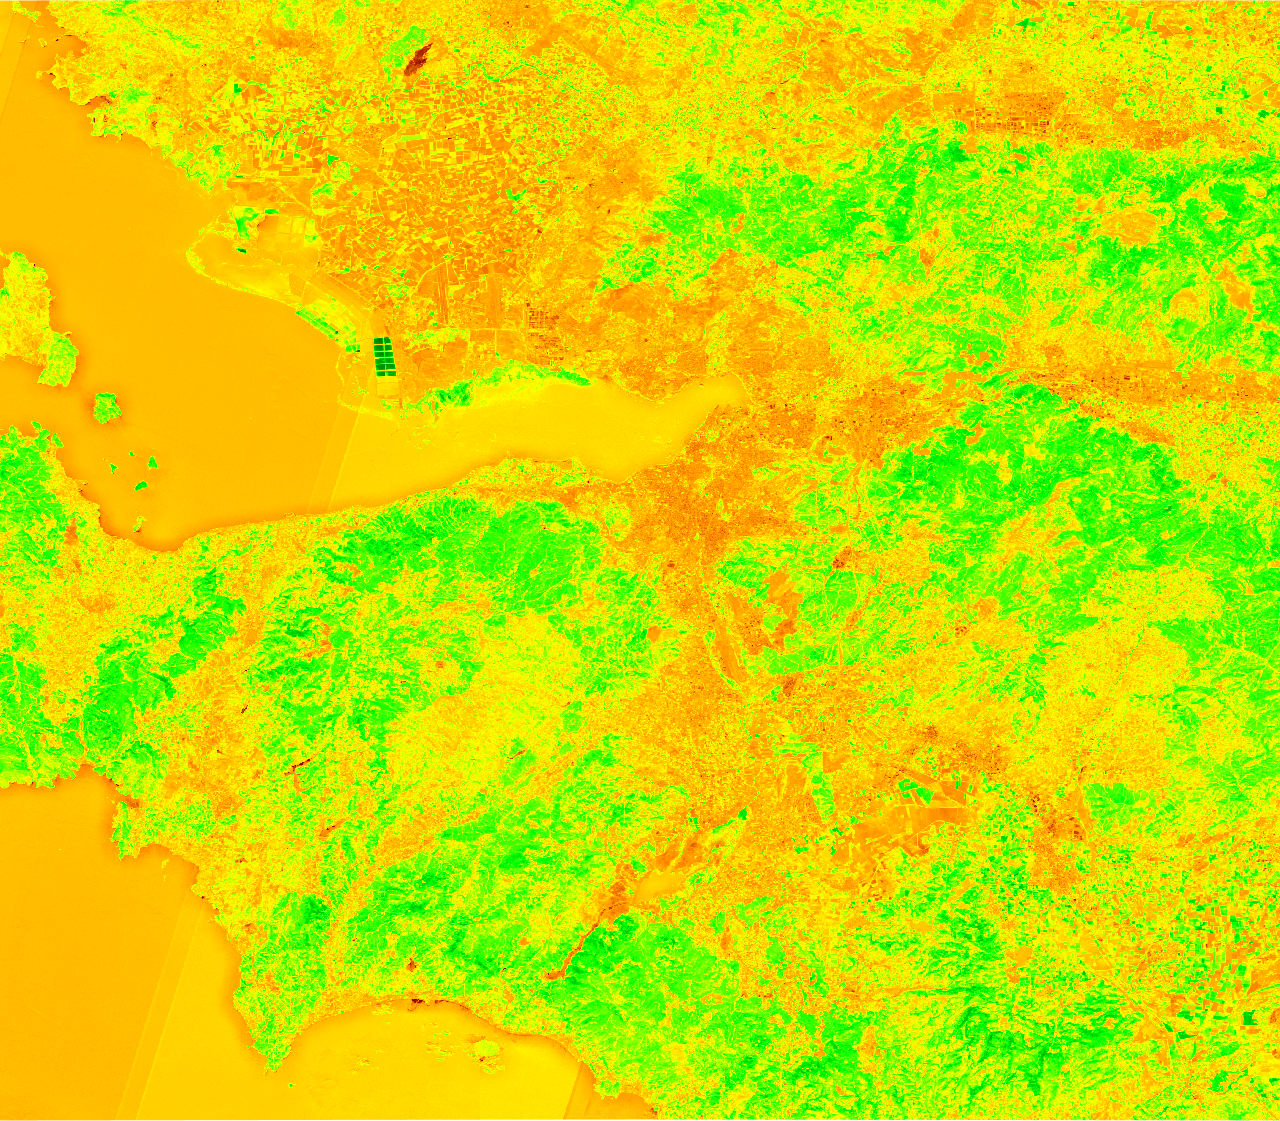
\includegraphics[width=\linewidth]{../results/pre_NBR.png}
    \caption{Öncesi NBR}
  \end{subfigure}\hfill
  \begin{subfigure}[b]{0.48\textwidth}
    \centering
    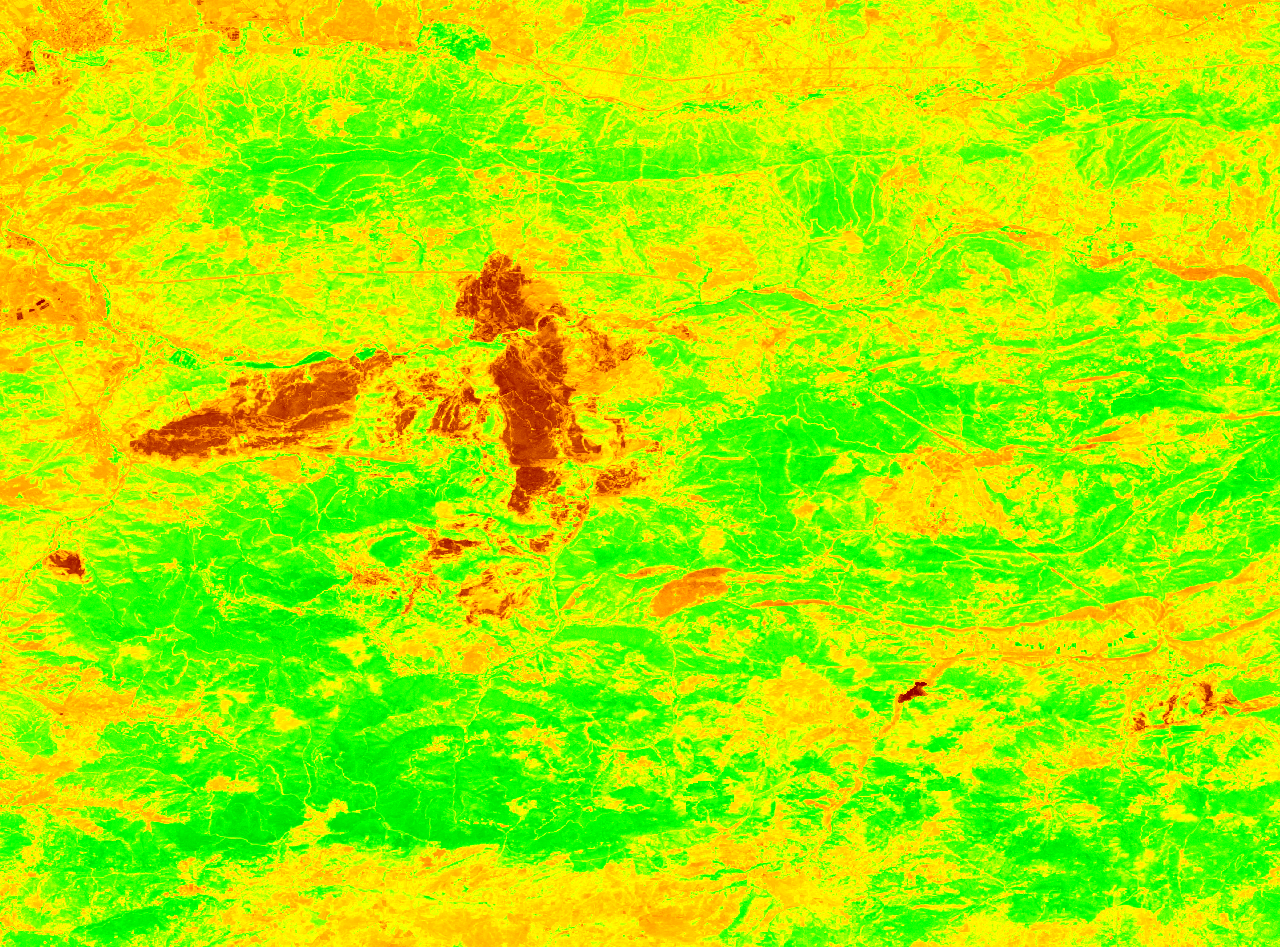
\includegraphics[width=\linewidth]{../results/post_NBR.png}
    \caption{Sonrası NBR}
  \end{subfigure}
  \caption{NBR karşılaştırması.}
\end{figure}
\FloatBarrier

\begin{figure}[H]
  \centering
  \begin{subfigure}[b]{0.48\textwidth}
    \centering
    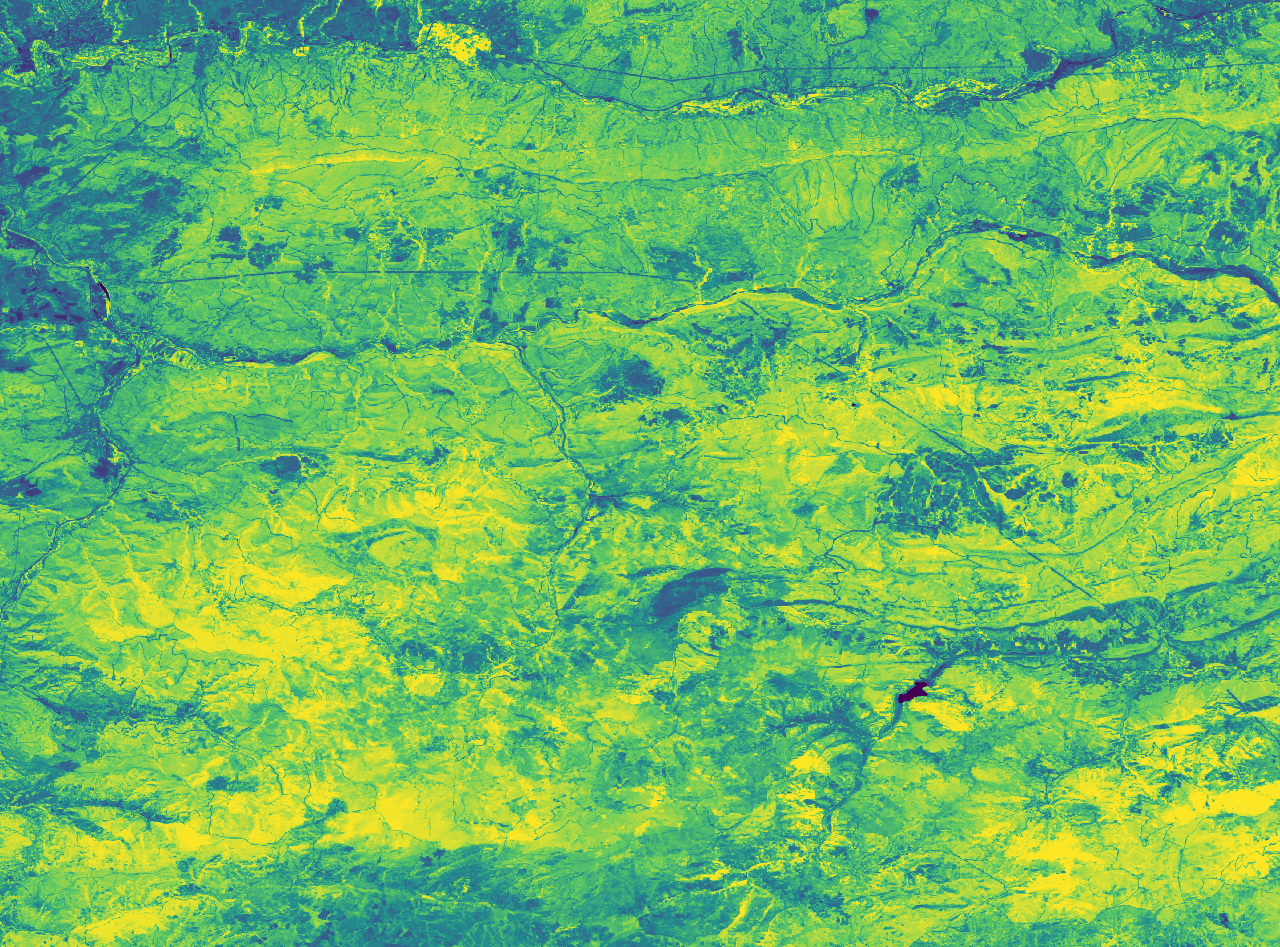
\includegraphics[width=\linewidth]{../results/pre_NDVI.png}
    \caption{Öncesi NDVI}
  \end{subfigure}\hfill
  \begin{subfigure}[b]{0.48\textwidth}
    \centering
    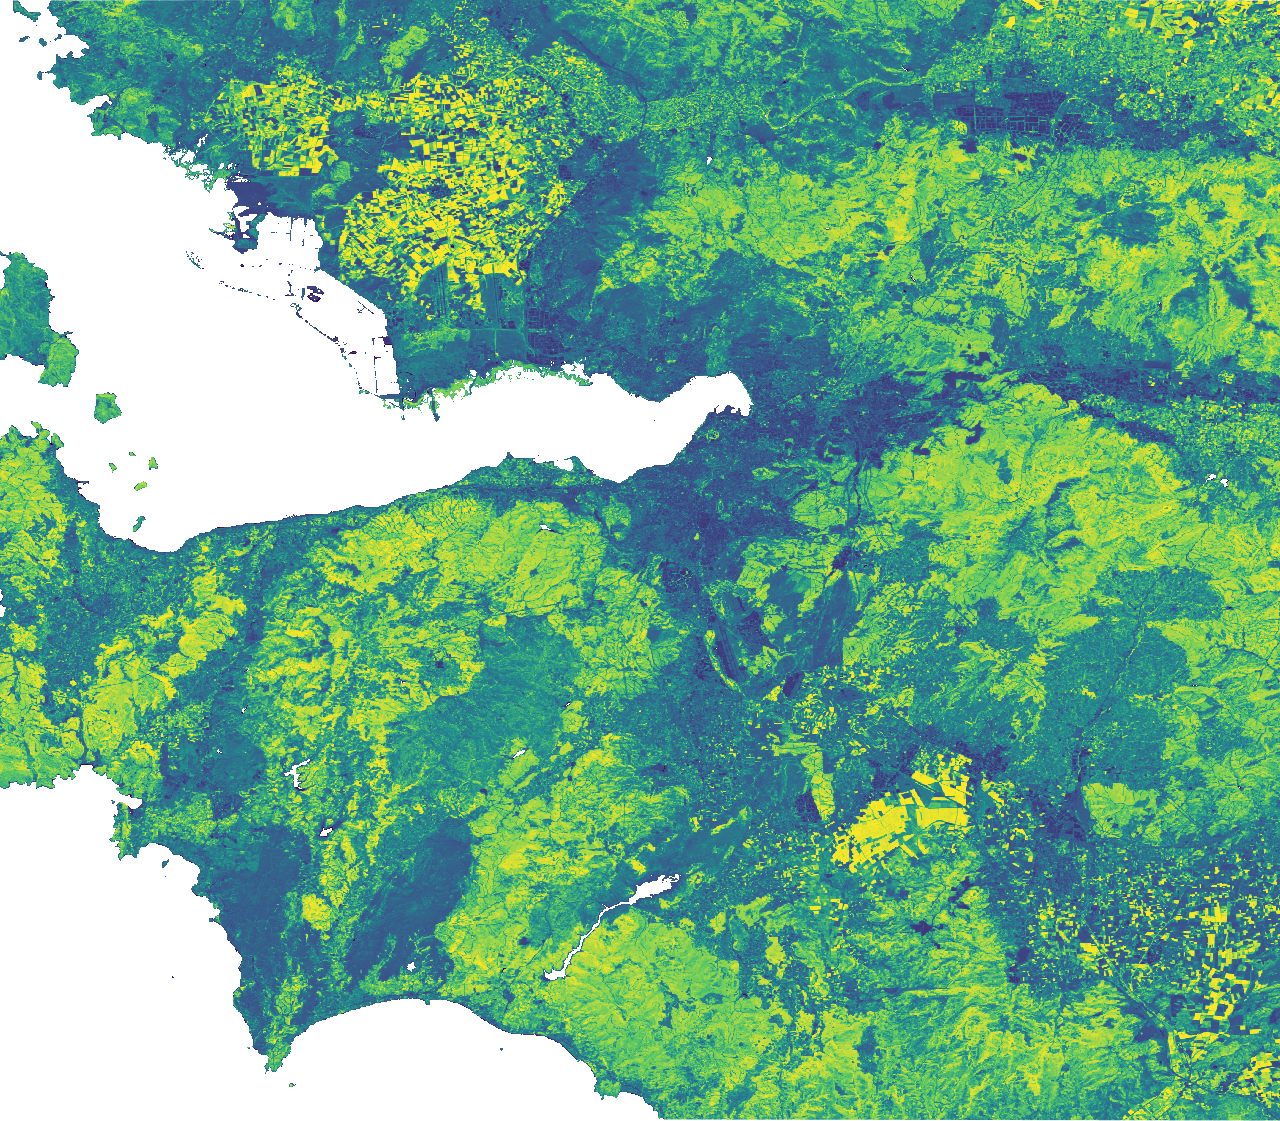
\includegraphics[width=\linewidth]{../results/post_NDVI.png}
    \caption{Sonrası NDVI}
  \end{subfigure}
  \caption{NDVI karşılaştırması.}
  \label{fig:ndvi}
\end{figure}
\FloatBarrier

\begin{figure}[H]
  \centering
  \begin{subfigure}[b]{0.48\textwidth}
    \centering
    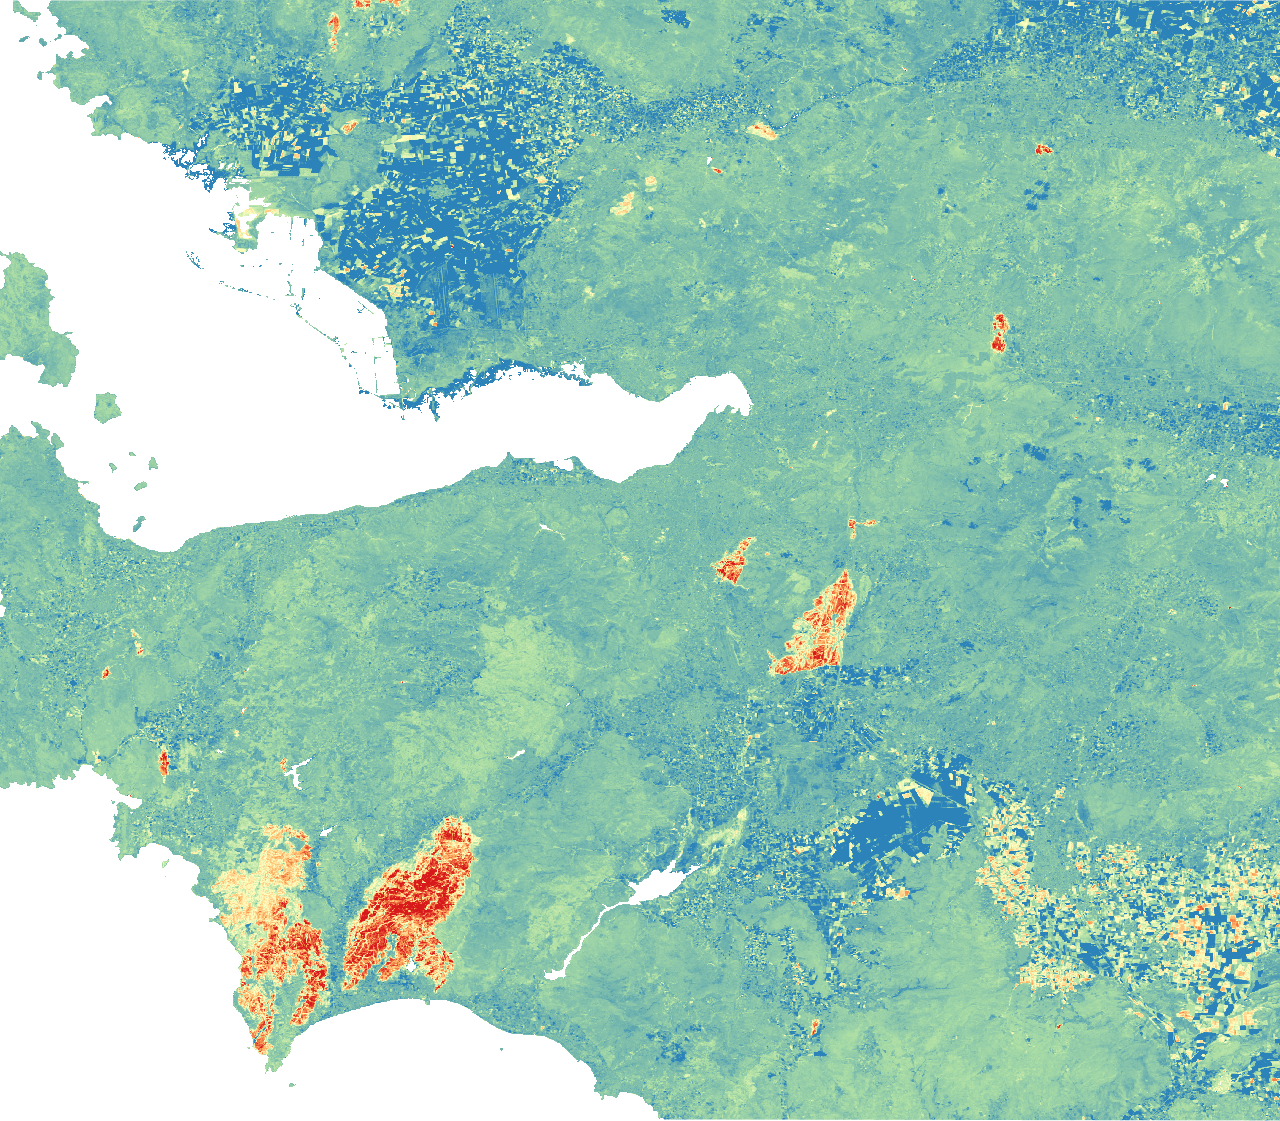
\includegraphics[width=\linewidth]{../results/dNBR.png}
    \caption{dNBR}
  \end{subfigure}\hfill
  \begin{subfigure}[b]{0.48\textwidth}
    \centering
    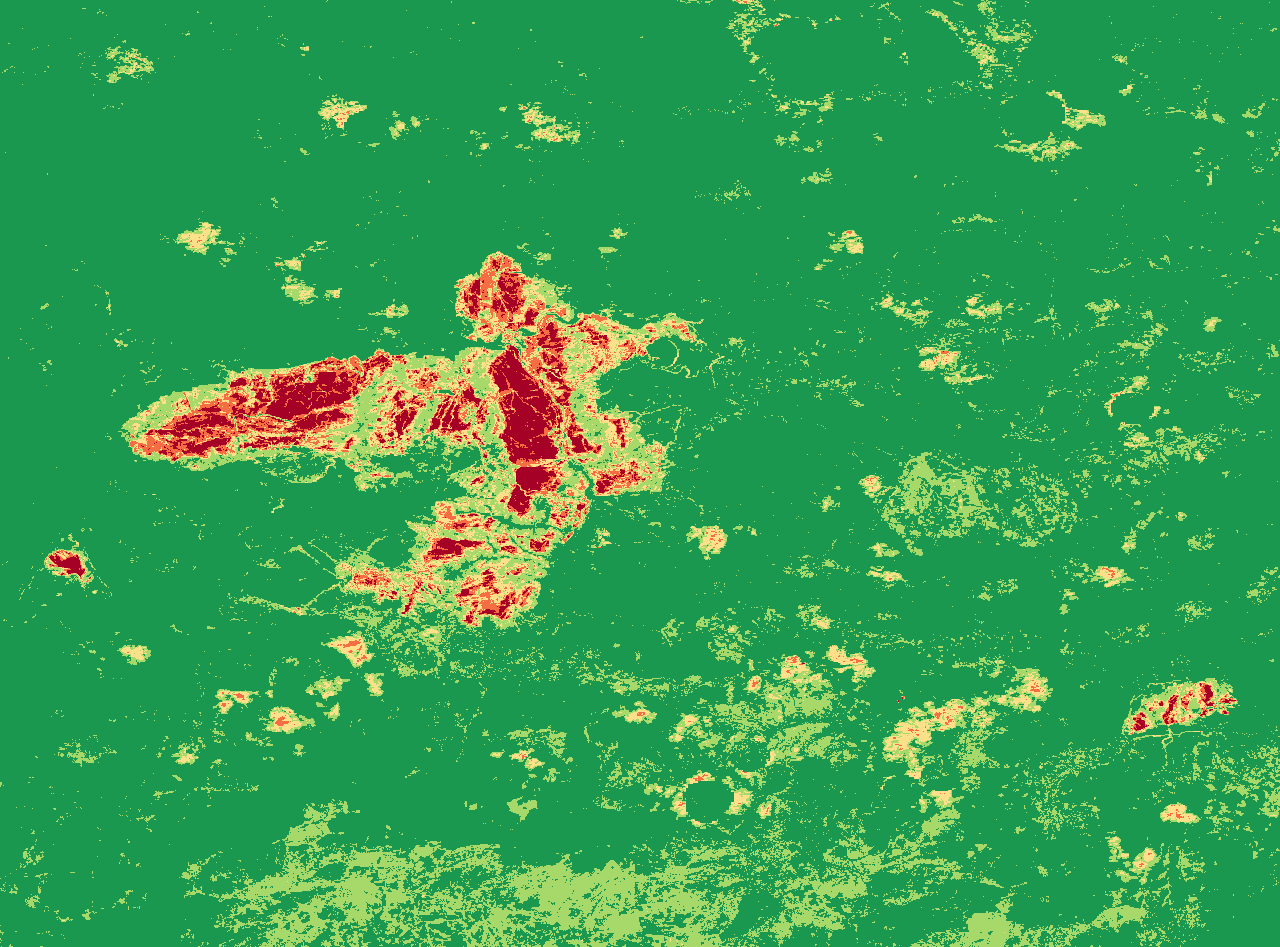
\includegraphics[width=\linewidth]{../results/severity.png}
    \caption{dNBR Şiddeti (0--4)}
  \end{subfigure}
  \caption{Fark analizi ve şiddet sınıfları.}
  \label{fig:diffs}
\end{figure}
\FloatBarrier

\section{Tartışma}
Uygulanan su/deniz ve kıyı filtreleri yalancı pozitifleri belirgin biçimde azaltmıştır. Bununla birlikte fenoloji farklılıkları ve aydınlatma geometrisi bölgesel önyargılar doğurabilir. Çalışmanın sonraki adımında RdNBR, MIRBI ve/veya Sentinel-1 SAR fark katmanlarıyla çoklu belirti kullanan bir eşikleme veya hafif bir denetimli sınıflandırma planlanmaktadır.

\section{Sınırlılıklar ve Belirsizlikler}
Bulut/duman kalıntıları, geometri/atmosfer artık hataları ve sabit eşiklerin genellenebilirliği sonuçları etkileyebilir. Eşiklerin AOI'ye göre kalibrasyonu, minimum yama alanı filtresinin ayarı ve mevsimsel uyum (önceki yıl aynı dönem referansı) önerilir.

\section{Sonuç}
Çalışma, Sentinel-2 tabanlı NDVI/NBR fark analizi ile İzmir AOI'sinde yangın etkisini düşük yanıklık şiddeti ve sınırlı alan kaybı ile tanımlamıştır. Maskeler ve kıyı tamponu kıyı/deniz kaynaklı yalancı değişimleri azaltarak yorum güvenilirliğini artırmıştır. Önerilen geliştirmelerle yöntemin sağlamlığı ve yerel doğruluğu daha da yükseltilebilir.

\end{document}

